\subsection{Risultati sperimentali}
Proponiamo alcuni risultati sperimentali ottenuti dal package Python contenente gli algoritmi per il calcolo della massima bisimulazione che abbiamo presentato nelle sezioni precedenti. Innanzitutto illustreremo brevemente l'ambiente e gli strumenti con cui sono state prese le misurazioni. Dopodichè presenteremo i risultati in forma di grafici, e tenteremo di evidenziare le differenze tra i vari algoritmi.

\subsubsection{Hardware e strumenti per le misura}
I risultati sono stati misurati su un computer con sistema operativo \emph{CentOS Linux}, architettura x86\_64, processore \emph{Intel(R) Core(TM) i7-4790 CPU} (4 cores, 3.60GHz), e memoria RAM da 16 GB. Per ottenere le misurazioni è stato utilizzato il package Python \emph{timeit}, che presenta alcune caratteristiche che lo rendono un valido strumento per la misurazione del tempo di esecuzione \cite{pythondocs}:
\begin{itemize}
    \item Utilizza la più precisa funzione disponibile sulla piattaforma per la misurazione del tempo trascorso;
    \item Disabilita il \emph{garbage collector}, che potrebbe intervenire in un momento casuale della misurazione introducendo rumore nei risultati;
    \item Esegue lo script preso in esame molte volte in modo da ridurre l'imprecisione dovuta a temporanei sovraccarichi della CPU o della RAM.
\end{itemize}

I dataset su cui abbiamo effettuato le misurazioni sono stati generati utilizzando alcune funzioni del package Python \emph{NetworkX} \cite{networkx}.

\subsubsection{Performance}
Consideriamo alcune tipologie differenti di grafi, e valutiamo il tempo necessario per l'esecuzione degli algoritmi che abbiamo implementato. Nei grafici utilizziamo lungo l'asse delle ascisse una scala data dal valore $|E| \log |V|$, che ci consente di visualizzare in modo più omogeneo i risultati lungo l'asse delle ordinate. Entrambi gli assi variano secondo una scala logaritmica.

\paragraph{Paige-Tarjan, Dovier-Piazza-Policriti} Cominciamo confrontando gli algoritmi di Paige-Tarjan e Dovier-Piazza-Policriti: ci aspettiamo che quest'ultimo risulti asintoticamente più conveniente. Per grafi piccoli invece dovrebbe risultare vincitore l'algoritmo di Paige-Tarjan visto che non richiede l'elaborazione preliminare del rango.

Cominciamo l'esposizione dei risultati con la categoria degli ``alberi bilanciati'', ovvero grafi che possono essere rappresentati nella forma esposta nella Figura \ref{fig:balanced_tree}. Essi sono caratterizzati da due parametri:
\begin{itemize}
    \item \emph{depth}: il numero di livelli (senza contare la \emph{root});
    \item \emph{branching factor}: il numero di successori di ogni nodo (ad eccezione dei nodi nell'ultimo livello).
\end{itemize}

Generiamo grafi di questo tipo tramite la funzione \verb|balanced_tree| di \emph{NetworkX}, che appunto prende in input questi due parametri.

\begin{figure}
    \centering
    \begin{subfigure}[b]{0.4\textwidth}
        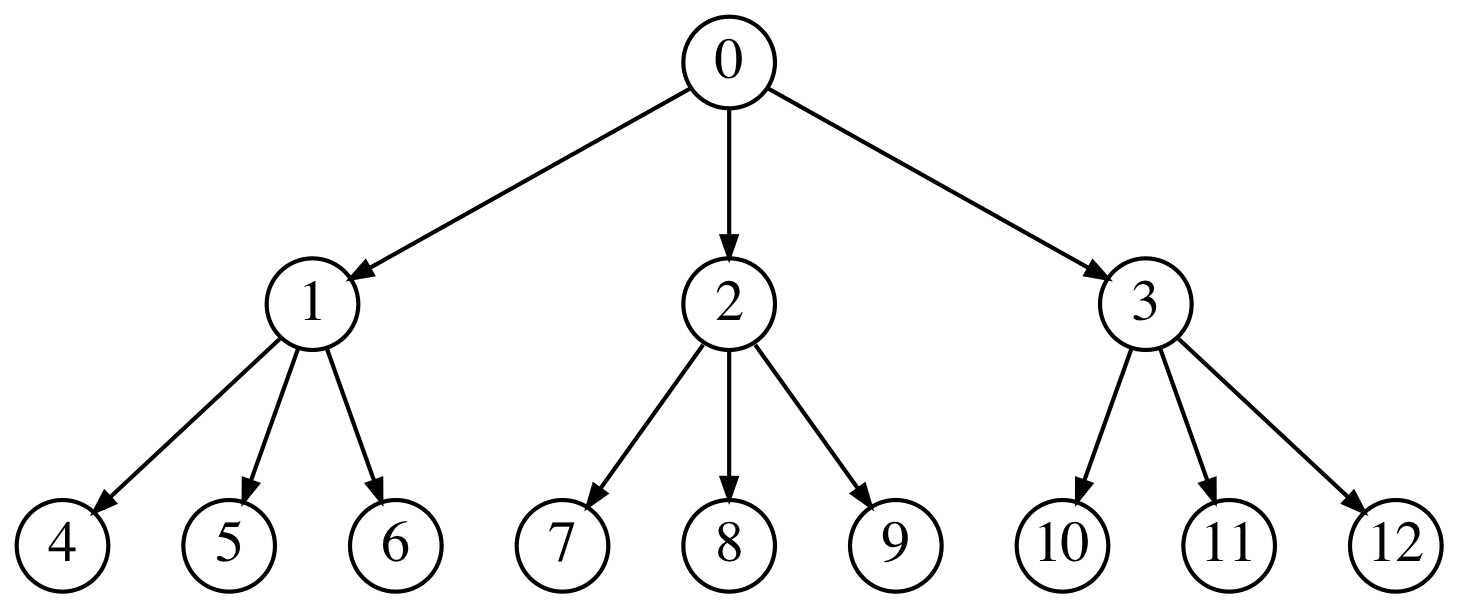
\includegraphics[width=\textwidth]{./sezione3/experimental_results/plots/tree_graph.png}
        \caption{Un albero bilanciato, \emph{depth}=2, \emph{branching factor}=3.}
        \label{fig:balanced_tree}
    \end{subfigure}
    \qquad
    \begin{subfigure}[b]{0.1\textwidth}
        \centering
        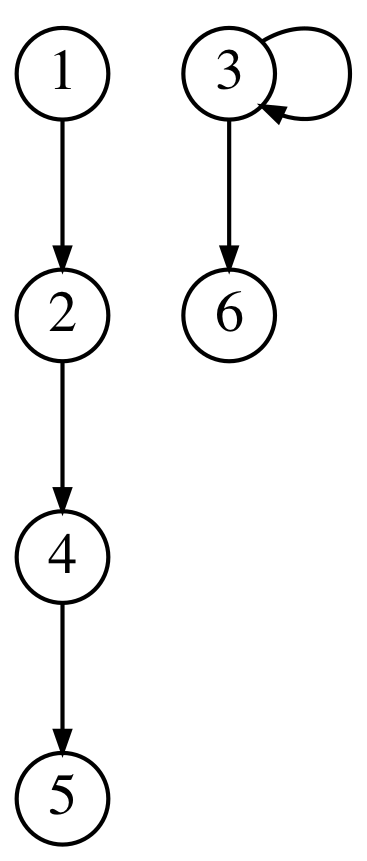
\includegraphics[width=\textwidth]{./sezione3/experimental_results/plots/hopcroft_graph_1.png}
        \caption{Hopcroft, $n=2$}
        \label{fig:hopcroft_graph_1}
    \end{subfigure}
    \qquad \qquad
    \begin{subfigure}[b]{0.2\textwidth}
        \centering
        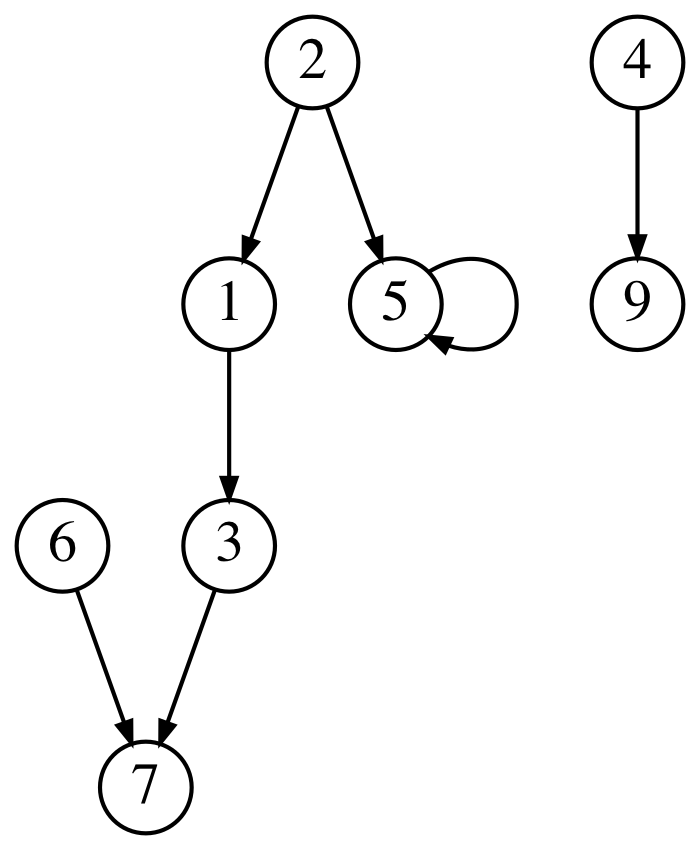
\includegraphics[width=\textwidth]{./sezione3/experimental_results/plots/hopcroft_graph_2.png}
        \caption{Hopcroft, $n=3$}
        \label{fig:hopcroft_graph_2}
    \end{subfigure}
    \caption{Tipologie di grafi su cui abbiamo testato gli algoritmi di Dovier-Piazza-Policriti e Paige-Tarjan.}
\end{figure}

Dalla Figura \ref{fig:tree_exp_result} possiamo osservare che asintoticamente l'algoritmo di Dovier-Piazza-Policriti è asintoticamente più efficiente, a partire da un certo valore di $|E| \log |V|$. Sebbene infatti la metodologia sia più ``rifinita'' dell'approccio di Paige-Tarjan, lo sforzo iniziale per il calcolo del rango è apprezzabile, soprattutto se consideriamo il linguaggio in cui l'algoritmo è stato implementato. Abbiamo però la conferma che per valori alti di $|E| \log |V|$, per questa tipologia di grafo, si ottengono i risultati previsti.

\begin{figure}
    \begin{subfigure}[t]{0.5\textwidth}
        \begin{tikzpicture}
            \begin{axis}[
                axis on top,
                width=\textwidth,
                ytick style={draw=none},
                xtick style={draw=none},
                xmode=log,
                ymode=log,
                grid=major
            ]
            \addplot table[x=x,y=y] {experiments/time/tree/pta.txt};
            \label{fig:pta_line_tree}
            \addplot table[x=x,y=y] {experiments/time/tree/fba.txt};
            \label{fig:fba_line_tree}
            \end{axis}
        \end{tikzpicture}
        \caption{Alberi bilanciati con \emph{depth} e \emph{branching factor} variabili.}
        \label{fig:tree_exp_result}
    \end{subfigure}
    \begin{subfigure}[t]{0.5\textwidth}
        \begin{tikzpicture}
            \begin{axis}[
                axis on top,
                width=\textwidth,
                ytick style={draw=none},
                xtick style={draw=none},
                grid=major,
                xmode=log,
                ymode=log
            ]
            \addplot table[x=x,y=y] {experiments/time/hopcroft/pta.txt};
            \label{fig:pta_line_hopcroft}
            \addplot table[x=x,y=y] {experiments/time/hopcroft/fba.txt};
            \label{fig:fba_line_hopcroft}
            \end{axis}
        \end{tikzpicture}
        \caption{Grafi della tipologia elaborata da Hopcroft, di dimensioni varie.}
        \label{fig:hopcroft_exp_result}
    \end{subfigure}
    \caption{Tempo di esecuzione degli algoritmi di Dovier-Piazza-Policriti (\ref*{fig:fba_line_tree}) e Paige-Tarjan (\ref*{fig:pta_line_tree}) sulle tipologie di grafo \ref{fig:balanced_tree} (a) e \ref{fig:hopcroft_graph_1}, \ref{fig:hopcroft_graph_2} (b). Lungo l'asse delle ascisse (logaritmico) abbiamo la quantità $|E|\log|V|$, mentre sull'asse delle ordinate (logaritmico) è riportato il tempo di esecuzione dell'algoritmo in secondi.}
\end{figure}

La seconda tiplogia di grafi che consideriamo è tratta dall'articolo in cui viene presentato l'algoritmo di Dovier-Piazza-Policriti, ed è un esempio di automa proposto originariamente da Hopcroft \cite{hopcroft}. Nelle Figure \ref{fig:hopcroft_graph_1} e \ref{fig:hopcroft_graph_2} ne visualizziamo alcune realizzazioni.

In Figura \ref{fig:hopcroft_exp_result} sono riportati i risultati ottenuti dagli algoritmi. Osserviamo nuovamente che l'algoritmo di Dovier-Piazza-Policriti risulta asintoticamente più conveniente anche in questo caso.

\paragraph{Dovier-Piazza-Policriti, Saha} Al fine di testare il tempo di esecuzione della nostra implementazione dell'algoritmo incrementale abbiamo esaminato una famiglia di alberi bilanciati del tipo mostrato nella Figura \ref{fig:balanced_tree}, per alcuni valori dei parametri \emph{depth}, \emph{branching factor}. Per questi grafi abbiamo considerato l'aggiunta di alcuni archi che riteniamo essere un valido insieme di \emph{test case} per l'algoritmo.

Definiamo innanzitutto la seguente funzione:
\begin{align*}
    L: V \times \mathbb{N} \to V, \qquad L(v, d) = ``&\text{Un nodo scelto casualmente tra i successori di $v$}\\
    &\text{ad un livello distante $d$ dal livello di $v$}''
\end{align*}

Abbiamo implementato questa funzione per mezzo di un ciclo, ed abbiamo scelto sempre il nodo più a sinistra tra tutti i candidati allo stesos livello (la scelta è ininfluente ai fini dell'esperimento).

Ad ogni realizzazzione dell'albero bilanciato aggingiamo i seguenti archi:
\begin{enumerate}
    \item $e_1 = \langle L(1, 2), 1 \rangle$;
    \item $e_2 = \langle L(1, 3), 1 \rangle$;
    \item $e_3 = \langle L(1, 4), 1 \rangle$;
    \item $e_4 = \langle L(1, 5), 1 \rangle$;
\end{enumerate}

Si osservi che la sorgente dell'arco si sposta verso il basso all'aumentare dell'indice dell'arco aggiunto. Poichè l'algoritmo di Saha visita ricorsivamente tutta la contro-immagine della sorgente dell'arco, ci aspettiamo di osservare nei risultati sperimentali un peggioramento del tempo di esecuzione all'aumentare dell'indice dell'arco aggiunto.

\begin{figure}[H]
    \centering
        \begin{subfigure}[b]{0.49\textwidth}
            \begin{tikzpicture}
                \begin{axis}[
                    axis on top,
                    width=\textwidth,
                    ytick style={draw=none},
                    xtick style={draw=none},
                    grid=major,
                    xmode=log,
                    ymode=log
                ]
                \addplot table[x=x,y=y] {experiments/time/tree_saha/fba0.txt};
                \label{fig:fba_line_saha}
                \addplot table[x=x,y=y] {experiments/time/tree_saha/sah0.txt};
                \label{fig:saha_line_saha}
                \end{axis}
            \end{tikzpicture}
            \caption{Arco $e_1$}
            \label{fig:saha_1_result}
        \end{subfigure}
        \begin{subfigure}[b]{0.49\textwidth}
            \begin{tikzpicture}
                \begin{axis}[
                    axis on top,
                    width=\textwidth,
                    ytick style={draw=none},
                    xtick style={draw=none},
                    grid=major,
                    xmode=log,
                    ymode=log%
                ]
                \addplot table[x=x,y=y] {experiments/time/tree_saha/fba1.txt};
                \addplot table[x=x,y=y] {experiments/time/tree_saha/sah1.txt};
                \end{axis}
            \end{tikzpicture}
            \caption{Arco $e_2$}
            \label{fig:saha_2_result}
        \end{subfigure}\\
        \begin{subfigure}[b]{0.49\textwidth}
            \begin{tikzpicture}
                \begin{axis}[
                    axis on top,
                    width=\textwidth,
                    ytick style={draw=none},
                    xtick style={draw=none},
                    grid=major,
                    xmode=log,
                    ymode=log
                ]
                \addplot table[x=x,y=y] {experiments/time/tree_saha/fba2.txt};
                \addplot table[x=x,y=y] {experiments/time/tree_saha/sah2.txt};
                \end{axis}
            \end{tikzpicture}
            \caption{Arco $e_3$}
            \label{fig:saha_3_result}
        \end{subfigure}
        \begin{subfigure}[b]{0.49\textwidth}
            \begin{tikzpicture}
                \begin{axis}[
                    axis on top,
                    width=\textwidth,
                    ytick style={draw=none},
                    xtick style={draw=none},
                    grid=major,
                    xmode=log,
                    ymode=log
                ]
                \addplot table[x=x,y=y] {experiments/time/tree_saha/fba3.txt};
                \addplot table[x=x,y=y] {experiments/time/tree_saha/sah3.txt};
                \end{axis}
            \end{tikzpicture}
            \caption{Arco $e_4$}
            \label{fig:saha_4_result}
        \end{subfigure}
    \caption{Tempo di esecuzione degli algoritmi di Dovier-Piazza-Policriti (\ref*{fig:fba_line_saha}) e Saha (\ref*{fig:saha_line_saha}) in seguito all'aggiunta di diversi tipi di arco, su alberi bilanciati con \emph{depth} e \emph{branching factor} variabili. Lungo l'asse delle ascisse varia la quantità $|E|\log|V|$, mentre l'asse delle ordinate corrisponde al tempo di esecuzione dell'algoritmo in secondi.}
    \label{fig:saha_result}
\end{figure}

L'esperimento dunque è stato condotto secondo questi passaggi:
\begin{itemize}
    \item Esecuzione dell'algoritmo di Dovier-Piazza-Policriti sul grafo in seguito all'aggiunta di un arco $e_i, i \in \{1,2,3,4\}$;
    \item Calcolo della massima bisimulazione del grafo prima della modifica;
    \item Aggiornamento della massima bisimulazione calcolata nel punto 2. dopo l'aggiunta del nuovo arco tramita l'algoritmo incrementale.
\end{itemize}

I risultati sono visualizzati nella Figura \ref{fig:saha_result}. Si osservi che in tutti i casi che abbiamo considerato l'algoritmo di Dovier-Piazza-Policriti impiega più tempo asintoticamente, come previsto.

Questa visualizzazione non ci consente di controllare la sensibilità dell'algoritmo incrementale alla tipologia di arco considerata. Nella Figura \ref{fig:saha_depends_cycle} è riportato l'andamento per $i \in \{2,3,4\}$ della funzione $T_i(G) - T_1(G)$, con $T_k(G)$ definita come segue:
\begin{align*}
    T_k(G) = ``&\text{tempo di esecuzione in secondi dell'algoritmo di Saha}\\
    &\text{in seguito all'aggiunta di } e_k''
\end{align*}

\begin{figure}[H]
    \begin{tikzpicture}
        \definecolor{color1}{rgb}{0.75,0,0.75}
        \definecolor{color0}{rgb}{0,0.75,0.75}
        \begin{axis}[
            axis on top,
            width=\textwidth,
            height=6cm,
            ytick style={draw=none},
            xtick style={draw=none},
            grid=major,
            legend cell align={left},
            legend style={font=\small, fill=white,opacity=0.8},
            legend pos=south west,
            tick pos=both,
            xtick style={color=black},
            ytick style={color=black},
            xlabel={$|E|\log|V|$},
            ylabel={Secondi},
            grid style={line width=.1pt, draw=gray!10},
            xmode=log,
            ymode=log
        ]
        \addplot table[x=x,y=y] {experiments/time/tree_saha/saha_diff0.txt};
        \label{fig:saha_diff_0}
        \addplot table[x=x,y=y] {experiments/time/tree_saha/saha_diff1.txt};
        \label{fig:saha_diff_1}
        \addplot table[x=x,y=y] {experiments/time/tree_saha/saha_diff2.txt};
        \label{fig:saha_diff_2}
        \end{axis}
    \end{tikzpicture}
    \caption{Differenza tra il tempo di esecuzione dell'algoritmo di Saha dopo l'aggiunta dell'arco $e_1$ e gli archi $e_2$ (\ref*{fig:saha_diff_0}), $e_3$ (\ref*{fig:saha_diff_1}), $e_4$ (\ref*{fig:saha_diff_2}).}
    \label{fig:saha_depends_cycle}
\end{figure}

\accente evidente che l'arco $e_4$ risulta il più pesante da aggiungere, risultato facilmente prevedibile dalle caratteristiche dell'algoritmo incrementale.

\subsubsection{Dimensione della massima bisimulazione}
Terminiamo la sezione relativa ai risultati sperimentali con un'ultima analisi che potrebbe essere di qualche interesse nella prospettiva di ciò che abbiamo presentato nella Sezione \ref{sec:applications}. Consideriamo l'andamento del numero di classi di equivalenza nella massima bisimulazione per grafi di Erdős-Rényi (o \emph{grafi binomiali}), ovvero grafi contenenti un numero arbitrario \verb|n| di nodi, per cui presa una coppia qualsiasi $u,v \in V$ si ha $\langle u,v\rangle \in E$ con probabilità \verb|p| $< 1$.
Considereremo valori piccoli di \verb|p|, in quanto avvicinandoci ad 1 otteniamo grafi sempre più ``completi'' di interesse molto basso nella pratica.

Nella Figura \ref{fig:bisi_size} abbiamo considerato tre diversi valori di \verb|n| (\verb|n=10| nella Figura \ref*{fig:bisi_dim_10}, \verb|n=100| nella Figura \ref*{fig:bisi_dim_100}, \verb|n=1000| nella Figura \ref*{fig:bisi_dim_1000}); inoltre abbiamo considerato quattro valori per \verb|p|: 0.01, 0.05, 0.1, 0.2.

\begin{figure}[H]
    \makebox[\textwidth][c]{
        \begin{subfigure}[b]{0.5\textwidth}
            \caption{$n=10$}
            \begin{tikzpicture}
                \begin{axis}[
                    axis on top,
                    width=\textwidth,
                    tick pos=both,
                    xtick style={color=black},
                    ytick style={color=black},
                    grid=both
                ]
                \addplot[scatter, scatter/classes={
                    a={mark=asterisk,blue},
                    b={mark=diamond,red},
                    c={mark=square,green},
                    d={mark=triangle,yellow}
                    }, only marks, scatter src=explicit symbolic] table[y=y,meta=label] {experiments/dimension/dim/result10.txt};
                \end{axis}
            \end{tikzpicture}
            \label{fig:bisi_dim_10}
        \end{subfigure}
        \begin{subfigure}[b]{0.5\textwidth}
            \caption{$n=100$}
            \begin{tikzpicture}
                \begin{axis}[
                    axis on top,
                    width=\textwidth,
                    tick pos=both,
                    xtick style={color=black},
                    ytick style={color=black},
                    grid=both
                ]
                \addplot[scatter, scatter/classes={
                    a={mark=asterisk,blue},
                    b={mark=diamond,red},
                    c={mark=square,green},
                    d={mark=triangle,yellow}
                    }, only marks, scatter src=explicit symbolic] table[y=y,meta=label] {experiments/dimension/dim/result100.txt};
                \end{axis}
            \end{tikzpicture}
            \label{fig:bisi_dim_100}
        \end{subfigure}
        \begin{subfigure}[b]{0.5\textwidth}
            \caption{$n=1000$}
            \begin{tikzpicture}
                \begin{axis}[
                    axis on top,
                    width=\textwidth,
                    tick pos=both,
                    xtick style={color=black},
                    ytick style={color=black},
                    grid=both
                ]
                \addplot[scatter, scatter/classes={
                    a={mark=asterisk,blue},
                    b={mark=diamond,red},
                    c={mark=square,green},
                    d={mark=triangle,purple}
                    }, only marks, scatter src=explicit symbolic] table[y=y,meta=label] {experiments/dimension/dim/result1000.txt};
                    \label[a]{fig:bisi_size_1000_p001}
                    \label[b]{fig:bisi_size_1000_p005}
                    \label[c]{fig:bisi_size_1000_p01}
                    \label[d]{fig:bisi_size_1000_p02}
                \end{axis}
            \end{tikzpicture}
            \label{fig:bisi_dim_1000}
        \end{subfigure}
    }
    \caption{Numero di classi di equivalenza della massima bisimulazione per grafi generati in modo casuale, normalizzato rispetto al numero di nodi nel grafo. Ad ogni \emph{tick} sull'asse delle ascisse corrisponde un grafo generato in modo casuale con $p=0.01$ (\ref*{fig:bisi_size_1000_p001}), $p=0.05$ (\ref*{fig:bisi_size_1000_p005}), $p=0.1$ (\ref*{fig:bisi_size_1000_p01}), $p=0.2$ (\ref*{fig:bisi_size_1000_p02}). Lungo l'asse delle ordinate è riportato il numero di blocchi della bisimulazione massima.}
    \label{fig:bisi_size}
\end{figure}

Per ogni combinazione di \verb|n|,\verb|p| abbiamo generato 100 grafi binomiali con la funzione \verb|fast_gnp_random_graph| del pacchetto \emph{NetworkX}, e ne abbiamo calcolata la massima bisimulazione con l'algoritmo di \emph{Dovier-Piazza-Policriti}. Nei grafici abbiamo visualizzato la quantità $\frac{|V / \equiv|}{|V|}$, ovvero il rapporto tra il numero di classi di equivalenza nella massima bisimulazione ed il numero di nodi del grafo: questa quantità potrebbe essere considerata come il fattore di riduzione che otteniamo quanto sostuitiamo al grafo originale la sua contrazione secondo la massima bisimulazione.

Per \verb|n=10| la quantità che stiamo valutando varia molto tra 1 (10 classi di equivalenza, nessuna riduzione) e 0.1 (tutti i nodi sono bisimili, riduzione massima). Per valori più grandi la variabilità si riduce, e per \verb|n=1000| il fattore si schiaccia decisamente verso 0.001 (un'unica partizione).
